\documentclass[11pt]{report}

% Paquetes y configuraciones adicionales
\usepackage{graphicx}
\usepackage[export]{adjustbox}
\usepackage{caption}
\usepackage{float}
\usepackage{titlesec}
\usepackage{geometry}
\usepackage[hidelinks]{hyperref}
\usepackage{titling}
\usepackage{titlesec}
\usepackage{parskip}
\usepackage{wasysym}
\usepackage{tikzsymbols}
\usepackage{fancyvrb}
\usepackage{xurl}
\usepackage{hyperref}
\usepackage{subcaption}

\usepackage{listings}
\usepackage{xcolor}

\usepackage[spanish]{babel}

\newcommand{\subtitle}[1]{
  \posttitle{
    \par\end{center}
    \begin{center}\large#1\end{center}
    \vskip0.5em}
}

% Configura los márgenes
\geometry{
  left=2cm,   % Ajusta este valor al margen izquierdo deseado
  right=2cm,  % Ajusta este valor al margen derecho deseado
  top=3cm,
  bottom=3cm,
}

% Configuración de los títulos de las secciones
\titlespacing{\section}{0pt}{\parskip}{\parskip}
\titlespacing{\subsection}{0pt}{\parskip}{\parskip}
\titlespacing{\subsubsection}{0pt}{\parskip}{\parskip}

% Redefinir el formato de los capítulos y añadir un punto después del número
\makeatletter
\renewcommand{\@makechapterhead}[1]{%
  \vspace*{0\p@} % Ajusta este valor para el espaciado deseado antes del título del capítulo
  {\parindent \z@ \raggedright \normalfont
    \ifnum \c@secnumdepth >\m@ne
        \huge\bfseries \thechapter.\ % Añade un punto después del número
    \fi
    \interlinepenalty\@M
    #1\par\nobreak
    \vspace{10pt} % Ajusta este valor para el espacio deseado después del título del capítulo
  }}
\makeatother

% Configura para que cada \chapter no comience en una pagina nueva
\makeatletter
\renewcommand\chapter{\@startsection{chapter}{0}{\z@}%
    {-3.5ex \@plus -1ex \@minus -.2ex}%
    {2.3ex \@plus.2ex}%
    {\normalfont\Large\bfseries}}
\makeatother

% Configurar los colores para el código
\definecolor{codegreen}{rgb}{0,0.6,0}
\definecolor{codegray}{rgb}{0.5,0.5,0.5}
\definecolor{codepurple}{rgb}{0.58,0,0.82}
\definecolor{backcolour}{rgb}{0.95,0.95,0.92}

% Configurar el estilo para el código
\lstdefinestyle{mystyle}{
  backgroundcolor=\color{backcolour},   
  commentstyle=\color{codegreen},
  keywordstyle=\color{magenta},
  numberstyle=\tiny\color{codegray},
  stringstyle=\color{codepurple},
  basicstyle=\ttfamily\footnotesize,
  breakatwhitespace=false,         
  breaklines=true,                 
  captionpos=b,                    
  keepspaces=true,                 
  numbers=left,                    
  numbersep=5pt,                  
  showspaces=false,                
  showstringspaces=false,
  showtabs=false,                  
  tabsize=2
}

%==============================================================================
% Cosas para la documentación LateX
% % Sangría
% \setlength{\parindent}{1em}Texto

% % Quitar sangría
% \noindent

% % Punto
% \CIRCLE \ \ \textbf{Texto} \emph{algo}
% \begin{itemize}
%   \item \textbf{Negrita:} Texto
%   \item \textbf{Negrita:} Texto
% \end{itemize}

% % Introducir código
% \begin{center}
%   \begin{BVerbatim}
%     ... Código
%   \end{BVerbatim}
% \end{center}

% Poner una imagen
% \begin{figure}[H]
%   \centering
%   \includegraphics[scale=0.55]{img/}
%   \caption{Exportación de la base de datos en formato sql}
%   \label{fig:exportación de la base de datos en formato sql}
% \end{figure}

% Poner dos imágenes
% \begin{figure}[H]
%   \begin{subfigure}{0.5\textwidth}
%     \centering
%     \includegraphics[scale=0.45]{img/}
%     \caption{Texto imagen 1}
%   \end{subfigure}%
%   \begin{subfigure}{0.5\textwidth}
%     \centering
%     \includegraphics[scale=0.45]{img/}
%     \caption{Texto imagen 2}
%   \end{subfigure}
%   \caption{Texto general}
% \end{figure}

% % Poner una tabla
% \begin{table}[H]
%   \centering
%   \begin{tabular}{|c|c|c|c|}
%     \hline
%     \textbf{Campo 1} & \textbf{Campo 2} & \textbf{Campo 3} & \textbf{Campo 4} \\ \hline
%     Texto & Texto & Texto & Texto \\ \hline
%     Texto & Texto & Texto & Texto \\ \hline
%     Texto & Texto & Texto & Texto \\ \hline
%     Texto & Texto & Texto & Texto \\ \hline
%   \end{tabular}
%   \caption{Nombre de la tabla}
%   \label{tab:nombre de la tabla}
% \end{table}

% % Poner codigo de un lenguaje a partir de un archivo
% \lstset{style=mystyle}
% The next code will be directly imported from a file
% \lstinputlisting[language=Python]{code.py}

% “Texto entre comillas dobles”

%==============================================================================

\begin{document}

% Portada del informe
\title{Práctica 07: Diseño y simplificación de gramáticas}
\subtitle{Computabilidad y Algoritmia}
\author{Cheuk Kelly Ng Pante (alu0101364544@ull.edu.es)}
\date{29/10/2024}

\maketitle

\pagestyle{empty} % Desactiva la numeración de página para el índice

% Índice
\tableofcontents

% Nueva página
\cleardoublepage

\pagestyle{plain} % Vuelve a activar la numeración de página
\setcounter{page}{1} % Reinicia el contador de página a 1

% Se pide para cada ejercicio:
% 1. El enunciado del ejercicio.
% 2. Una breve explicacion de la gramatica diseñada, describiendo los criterios se-
% guidos durante el dise ̃no, as ́ı como las reglas y elementos que la componen.
% 3. Una imagen con la gram ́atica dise ̃nada en JFLAP.
% 4. Al menos tres ejemplos de cadenas que pueden ser generadas a partir de la
% gram ́atica (incluir cada  ́arbol de an ́alisis sint ́actico).
% 5. Una descripci ́on detallada del proceso, paso a paso, de simplificaci ́on de la
% gram ́atica junto con una verificaci ́on de que el resultado realizado de forma
% aut ́onoma coincide con el resultado obtenido con cada algoritmo en JFLAP

% Secciones del informe
% Capitulo 1
\chapter{Ejercicios de diseño de gramáticas}
\section{Diseñar una gramática independiente del contexto que genere el lenguaje \texorpdfstring{$L = \{a^n b^n \mid n \geq 0\}$}{L = \{a^n b^n | n >= 0\}}}
\begin{itemize}
  \item \textbf{Explicación de la gramática:} La gramática diseñada para el lenguaje $L = \{a^n b^n \mid n \geq 0\}$ sigue la siguiente estructura:
  \begin{itemize}
    \item $S \rightarrow aSb \mid \varepsilon$
  \end{itemize}
  \item \textbf{Imagen de la gramática en JFLAP:} La gramática diseñada en JFLAP se muestra en la siguiente figura:
  \begin{figure}[H]
    \centering
    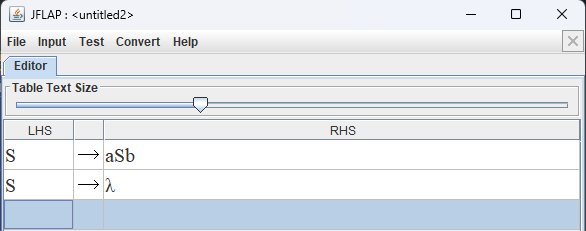
\includegraphics[scale=0.55]{img/grammar_01.png}
    \caption{Gramática diseñada en JFLAP para el lenguaje $L = \{a^n b^n \mid n \geq 0\}$}
  \end{figure}
  \item \textbf{Ejemplos de cadenas generadas:}
  \begin{itemize}
    \item \textbf{Cadena 1:} $aabb$
    \begin{itemize}
      \item \textbf{Árbol de análisis sintáctico:} El árbol de análisis sintáctico para la cadena $aabb$ se muestra en la siguiente figura:
      \begin{figure}[H]
        \centering
        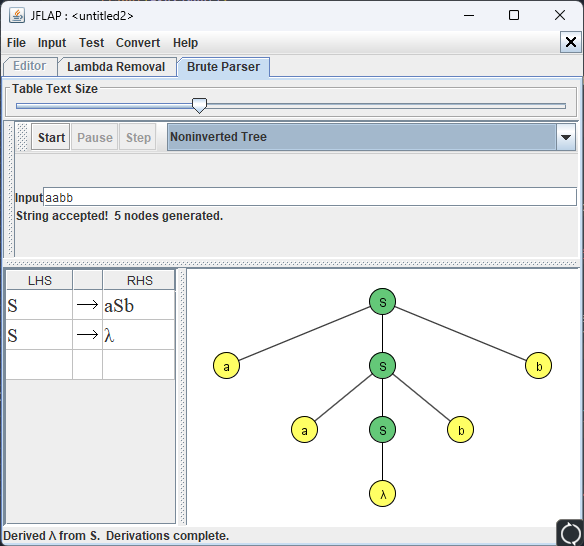
\includegraphics[scale=0.5]{img/grammar_01_tree_1.png}
        \caption{Árbol de análisis sintáctico para la cadena $aabb$}
        \label{fig:arbol1}
      \end{figure}
    \end{itemize}
    \item \textbf{Cadena 2:} $aaabbb$
    \begin{itemize}
      \item \textbf{Árbol de análisis sintáctico:} El árbol de análisis sintáctico para la cadena $aaabbb$ se muestra en la siguiente figura:
      \begin{figure}[H]
        \centering
        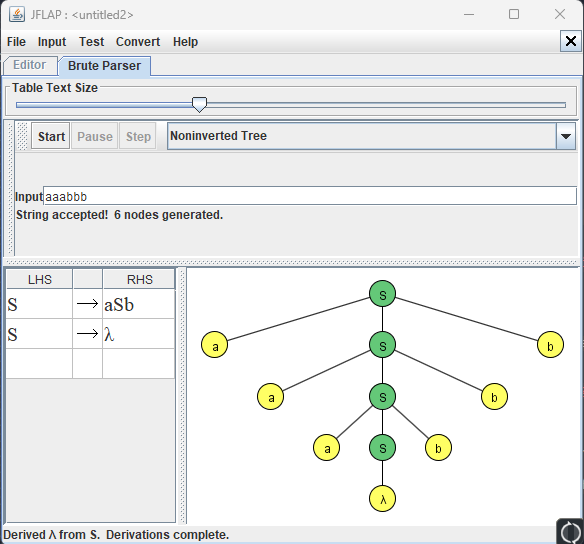
\includegraphics[scale=0.5]{img/grammar_01_tree_2.png}
        \caption{Árbol de análisis sintáctico para la cadena $aaabbb$}
        \label{fig:arbol2}
      \end{figure}
    \end{itemize}
    \item \textbf{Cadena 3:} $aaaaaabbbbbb$
    \begin{itemize}
      \item \textbf{Árbol de análisis sintáctico:} El árbol de análisis sintáctico para la cadena $aaaaaabbbbbb$ se muestra en la siguiente figura:
      \begin{figure}[H]
        \centering
        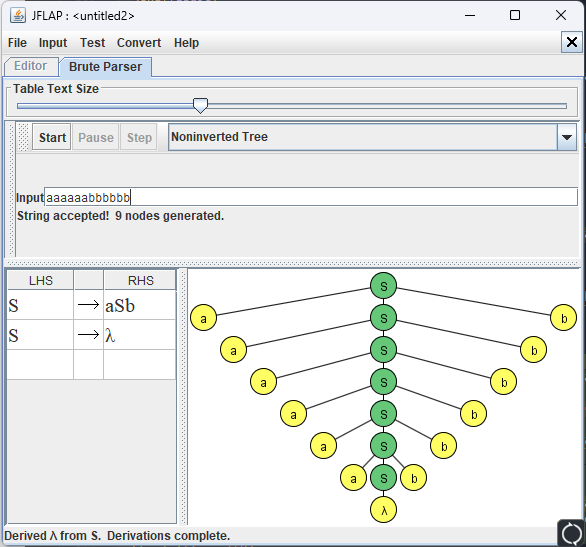
\includegraphics[scale=0.5]{img/grammar_01_tree_3.png}
        \caption{Árbol de análisis sintáctico para la cadena $aaaaaabbbbbb$}
        \label{fig:arbol3}
      \end{figure}
    \end{itemize}
  \end{itemize}
  \item \textbf{Imagen de la gramática simplificada en JFLAP:} La gramática simplificada en JFLAP se muestra en la siguiente figura:
  \begin{figure}[H]
    \centering
    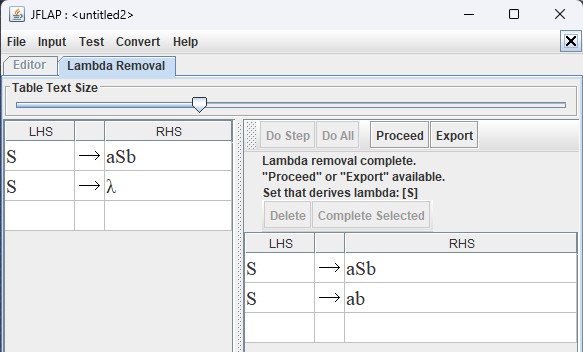
\includegraphics[scale=0.55]{img/grammar_01_simplified.png}
    \caption{Gramática simplificada en JFLAP para el lenguaje $L = \{a^n b^n \mid n \geq 0\}$}
    \label{fig:gramatica1_simplified}
  \end{figure}
\end{itemize}

\newpage

\section{Diseñar una gramática independiente del contexto que genere el lenguaje \texorpdfstring{$L = \{a^n b^m \mid n, m \geq 0, n \neq m\}$}{L = \{a^n b^m | n, m >= 0, n ≠ m\}}}
\begin{itemize}
  \item \textbf{Explicación de la gramática:} La gramática diseñada para el lenguaje $L = \{a^n b^m \mid n, m \geq 0, n \neq m\}$ sigue la siguiente estructura:
  \begin{itemize}
    \item $S \rightarrow aSb \mid A \mid B$
    \item $A \rightarrow aA \mid a$
    \item $B \rightarrow bB \mid b$
  \end{itemize}
  \item \textbf{Imagen de la gramática en JFLAP:} La gramática diseñada en JFLAP se muestra en la siguiente figura:
  \begin{figure}[H]
    \centering
    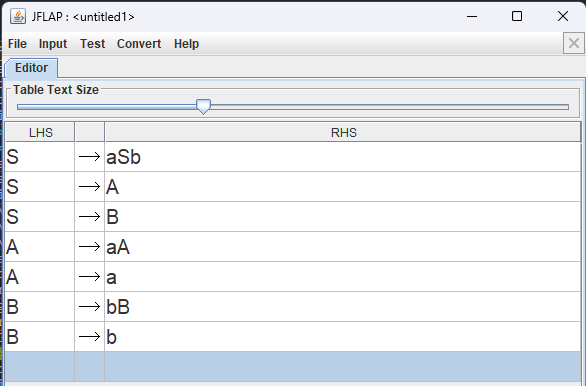
\includegraphics[scale=0.55]{img/grammar_02.png}
    \caption{Gramática diseñada en JFLAP para el lenguaje $L = \{a^n b^m \mid n, m \geq 0, n \neq m\}$}
  \end{figure}
  \item \textbf{Ejemplos de cadenas generadas:}
  \begin{itemize}
    \item \textbf{Cadena 1:} $aab$
    \begin{itemize}
      \item \textbf{Árbol de análisis sintáctico:} El árbol de análisis sintáctico para la cadena $aab$ se muestra en la siguiente figura:
      \begin{figure}[H]
        \centering
        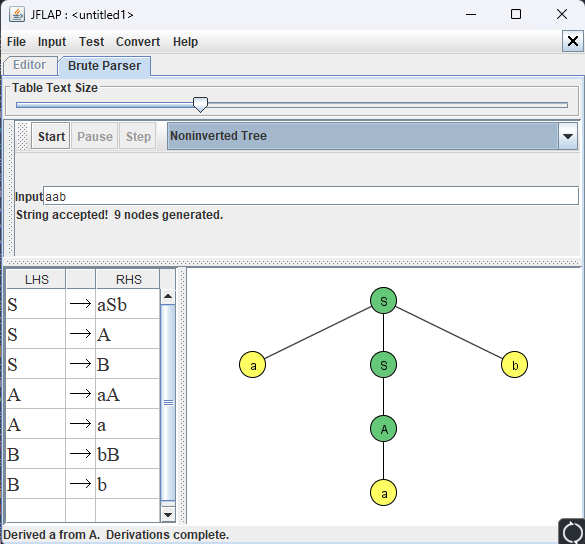
\includegraphics[scale=0.5]{img/grammar_02_tree_1.png}
        \caption{Árbol de análisis sintáctico para la cadena $aab$}
        \label{fig:arbol4}
      \end{figure}
    \end{itemize}
    \item \textbf{Cadena 2:} $ab$
    \begin{itemize}
      \item \textbf{Árbol de análisis sintáctico:} El árbol de análisis sintáctico para la cadena $ab$ se muestra en la siguiente figura:
      \begin{figure}[H]
        \centering
        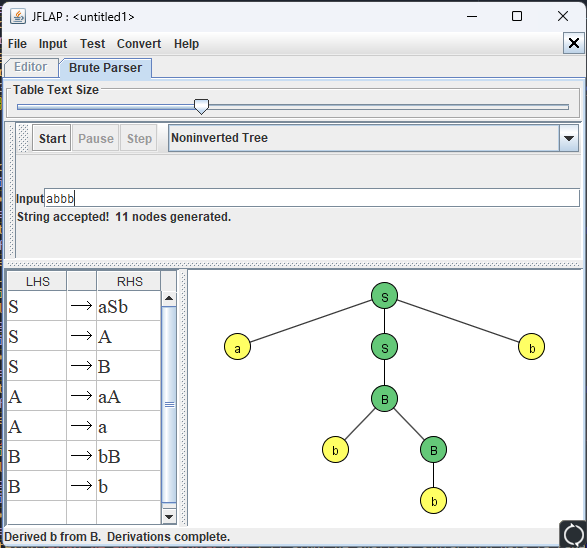
\includegraphics[scale=0.5]{img/grammar_02_tree_2.png}
        \caption{Árbol de análisis sintáctico para la cadena $ab$}
        \label{fig:arbol5}
      \end{figure}
    \end{itemize}
    \item \textbf{Cadena 3:} $aabb$
    \begin{itemize}
      \item \textbf{Árbol de análisis sintáctico:} El árbol de análisis sintáctico para la cadena $aabb$ se muestra en la siguiente figura:
      \begin{figure}[H]
        \centering
        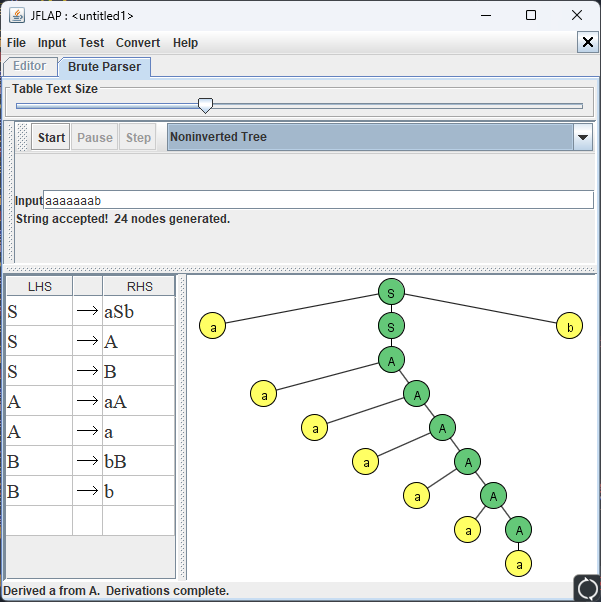
\includegraphics[scale=0.5]{img/grammar_02_tree_3.png}
        \caption{Árbol de análisis sintáctico para la cadena $aabb$}
        \label{fig:arbol6}
      \end{figure}
    \end{itemize}
  \end{itemize}
  \item \textbf{Imagen de la gramática simplificada en JFLAP:} La gramática simplificada en JFLAP se muestra en la siguiente figura:
  \begin{figure}[H]
    \centering
    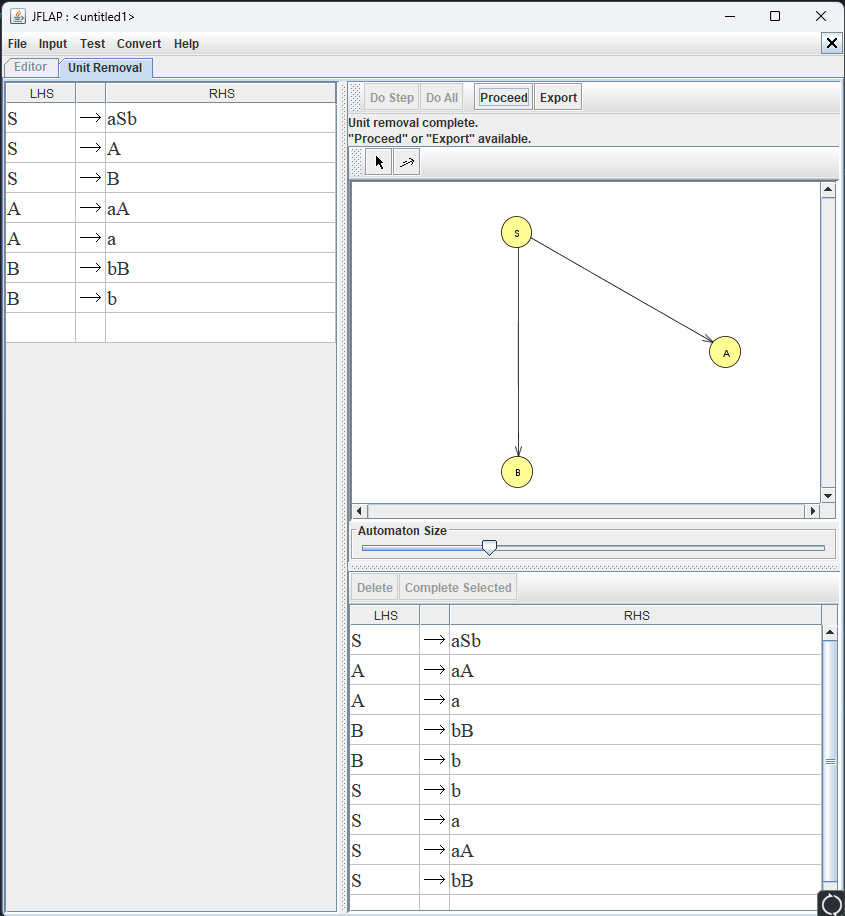
\includegraphics[scale=0.55]{img/grammar_02_simplified.png}
    \caption{Gramática simplificada en JFLAP para el lenguaje $L = \{a^n b^m \mid n, m \geq 0, n \neq m\}$}
    \label{fig:gramatica2_simplified}
  \end{figure}
\end{itemize}

\end{document}